\begin{figure}
    \centering
    %\tikzstyle{block} = [rectangle, rounded corners, text=black, text centered, draw=black, minimum height=.3in]
    %\tikzstyle{block} = [rectangle, rounded corners, text=black, text centered, draw=black,font=\scriptsize, minimum height=.35in, minimum width=.65in]
    \tikzstyle{block} = [rectangle, rounded corners, text=black, text centered, draw=black,font=\scriptsize, minimum width=1.2in, minimum height=.2in]
    \tikzstyle{line} = [-latex,draw=black,line width=.5, densely dotted]
    \tikzstyle{line2} = [latex-latex,draw=black,line width=.4, densely dashed]
    \tikzstyle{line3} = [-latex,draw=black,line width=.4, densely dotted]
    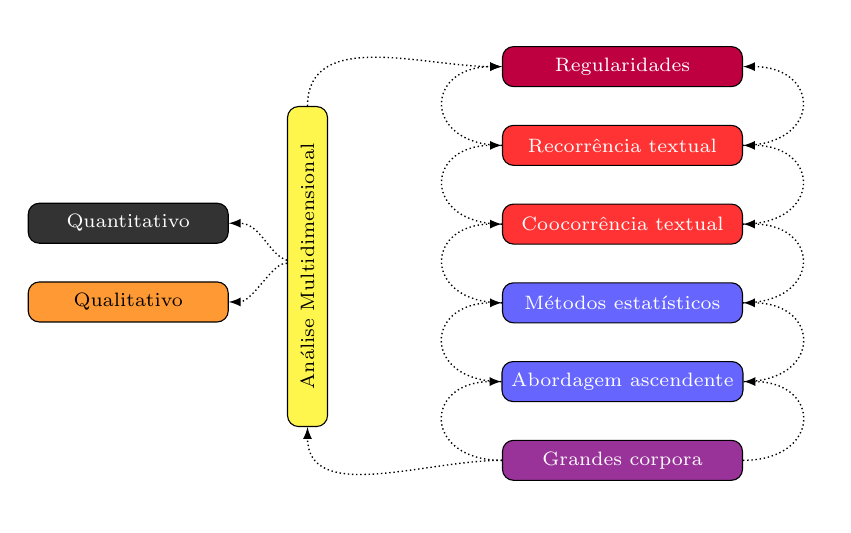
\begin{tikzpicture}
        \node[block,fill=purple!100,text=white, anchor=north] (regul) at (10,10) {Regularidades};
        \node[block,fill=red!80,text=white, anchor=north] (recur) at (10,9) {Recorrência textual};
        \node[block,fill=red!80,text=white, anchor=north] (cooc) at (10,8) {Coocorrência textual};
        \node[block,fill=blue!60,text=white, anchor=north] (stats) at (10,7) {Métodos estatísticos};
        \node[block,fill=blue!60,text=white, anchor=north] (bottomup) at (10,6) {Abordagem ascendente};
        \node[block,fill=violet!80,text=white, anchor=north] (corpora) at (10,5) {Grandes corpora};
        \node[block, fill=yellow!70, text=black, rotate=90, minimum width=1.6in] (compute) at (6,7.2) {Análise Multidimensional};
        \node[block,fill=black!80,text=white, anchor=east, minimum width=1in] (quant) at (5,7.75) {Quantitativo};
        \node[block,fill=orange!80,text=black, anchor=east, minimum width=1in] (qual) at (5,6.75) {Qualitativo};
        %\node[block, fill=purple!40, text=white, rotate=90, minimum width=1.6in] (mda) at (14,7.2) {Multi-Dimensional Analysis};
        %\node[block,fill=purple!10,text=black,text width=.75in, anchor=north, dashed] (underlying) at (10,9.75) {Underlying dimensions};
        \draw[line] (corpora.east) .. controls +(1,0) and +(1,0) .. (bottomup.east);
        \draw[line] (bottomup.east) .. controls +(1,0) and +(1,0) .. (stats.east);
        \draw[line] (stats.east) .. controls +(1,0) and +(1,0) .. (cooc.east);
        \draw[line] (cooc.east) .. controls +(1,0) and +(1,0) .. (recur.east);
        \draw[line] (recur.east) .. controls +(1,0) and +(1,0) .. (regul.east);
        \draw[line] (corpora.west) .. controls +(-1,0) and +(-1,0) .. (bottomup.west);
        \draw[line] (bottomup.west) .. controls +(-1,0) and +(-1,0) .. (stats.west);
        \draw[line] (stats.west) .. controls +(-1,0) and +(-1,0) .. (cooc.west);
        \draw[line] (cooc.west) .. controls +(-1,0) and +(-1,0) .. (recur.west);
        \draw[line] (recur.west) .. controls +(-1,0) and +(-1,0) .. (regul.west);
        \draw[line] (corpora) to[out=180, in=270] (compute.west);
        \draw[line] (compute.east) to[out=90, in=180] (regul);
        \draw[line] (compute) to [out=125, in=0] (quant);
        \draw[line] (compute) to [out=125, in=0] (qual);
        %\draw[line2] (cognition) to [in=270,out=270] (society);
        %\draw[line2] (cognition) .. controls +(0,-1) and +(0,-1) .. (society);
    \end{tikzpicture}
    %\footnotetext{Mostly.}
    \caption{Lexical Multi-Dimensional Analysis 2 \citep{berbersardinhaLexicalMultiDimensionalAnalysis2025}}
    \label{fig:lexical_md_analysis2}
\end{figure}
